Simulating cosmological structure has been of increased interest in the past decade. Simulating these structures can tell us about cosmological expansion \cite{cosmological-expansion-application}, galaxy formation \cite{galaxy-formation-application}, and dark matter halos \cite{dark-matter-application}. This leads us to a better understanding of cosmological parameters. However, the simulations need to be increasingly complex and detailed in order to make novel conclusions.

Simulating the behavior of an astrophysical system with a fine-granularity is computationally expensive. However, a technique known as \textbf{superresolution} may be able to reduce the cost by simulating the system at a coarse-granularity `big picture' and using some other method to reconstruct the fine-grain `details.' One could use superresolution to refine the resolution in space, time, or both, but I will use it for space.

Spatial superresolution was originally studied for videos. The hidden variable is the function from 2D-position to colors in the camera's perspective. Although it exists continuously, it is only sampled/observed discretely at pixel points.
Any movement between the subject and the observer in subsequent frames shifts the pixel grid slightly to yield a new sampling at \textit{different} gridpoints, as in \cref{classical-superresolution}.
Features which may have fallen in between pixels in one frame may fall right on a pixel in another frame (because the camera or the subject moved slightly), so the feature's existence in the first frame can be inferred.
This is the `information theoretical' basis for video superresolution given by Katsaggelos et al. \cite{synthesis-lecture}.

\begin{figure}[h!]
  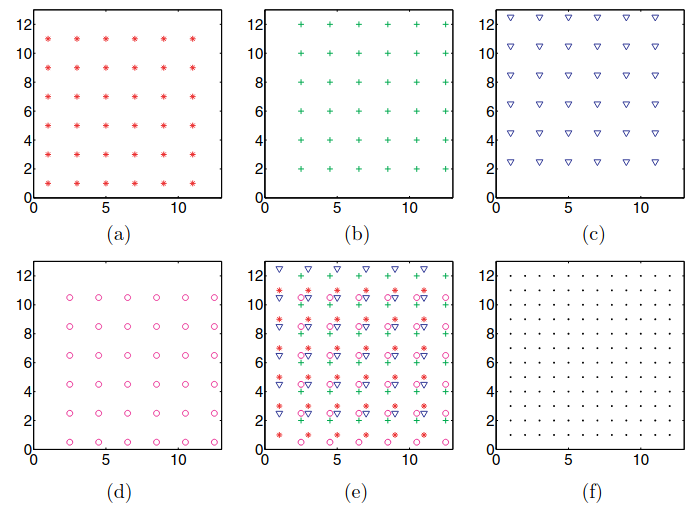
\includegraphics[width=4in]{classical-superresolution.png}
  \caption{Low-resolution images (a), (b), (c), and (d), when overlayed, sample the underlying phenomenon at the points in (e). This set of low-resolution images can synthesize a higher-resolution image, (f), with classical superresolution.}
  \label{classical-superresolution}
\end{figure}

However, in superresolution for simulations, the hidden variable is the high-granularity simulation, and it only exists discretely. There are no features in the high-granularity simulation to recover finer than the fine-grain gridpoints. This same theoretical justification does not apply, but perhaps another does: given the ergodic principle, every patch of space should have some patch in the training set that looks similar. In theory, superresolution can work by saving computational resources by learning what happens to small patches of space in the \textbf{training phase} and interpolating a novel patch based in the \textbf{prediction phase} (see \cref{gan-for-superresolution}a.). While neural networks are universal function approximators, a neural network can be more computationally expensive than the function it was trained to approximate (in this case, the fine-grained fluid dynamic simulation); in order to be worthwhile, high-resolution inference (\cref{gan-for-superresolution}b.) has to be cheaper than a bona fide high-resolution simulation (\cref{gan-for-superresolution}c.).

\begin{figure}[h!]
  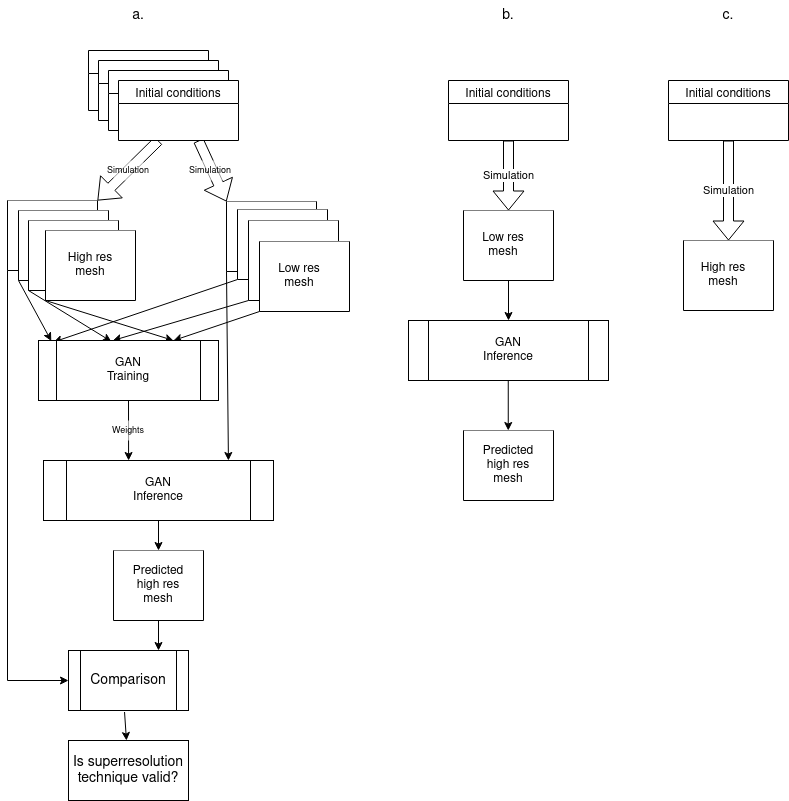
\includegraphics[width=\textwidth]{GAN_for_superresolution.drawio.png}
  \caption{a. shows training and validation of the GAN; b. shows usage of the GAN; c. shows the process the GAN can replace.}
  \label{gan-for-superresolution}
\end{figure}

Some \cite{superresolving-halos,survey} have suggested using a generative adverserial neural network (GAN) for superresolution. GANs were first proposed by Ian Goodfellow in 2014 \cite{GAN}. Suppose one wants to generate data in \(B\) based on a set of parameters \(A\). A GAN consists of two networks: a generator \(G: A \to B\) and a discriminator \(D: A \cross B \to [0, 1]\). To train a GAN, one needs genuine examples, \(R \subseteq A \cross B\). 
Intuitively, discriminator is trained to tell apart the genuine examples (elements of \(R\)), while the generator is trained to trick the descriminator with \((a, G(a))\) for \(a \in A\).
Let \[L(G, D) = \mathbb E [\log D(a, b) | (a, b) \in R] + \mathbb E [\log(1 - D(G(a))) | a \in A]\]
where \(\mathbb E(f(x) | x \in X)\) is the expected value of \(f(x)\).
Training runs in epochs where every even epoch updates the descriminator to maximize \(L\), while every odd epoch updates the generator to minimize \(L\), finding the \(\min\limits_G \max\limits_D L(G, D)\).

A Nash Equilibrium for this system is guaranteed to exist, although training might not reach it in a reasonable time. See \cite{GAN-explainer} for more background.
Once training is done, one can throw away \(D\) and use \(G\) to map from \(A\) to \(B\), hopefully in a realistic way.
In our case, \(A\) will be the low-resolution images, and \(B\) will be the high-resolution images.

Schaurecker et al. \cite{superresolving-halos} apply a generative adverserial network to superresolution for cosmological structure in a dark-matter simulation called Illustris \cite{Illustris}. Rather than an \textit{Eulerian} mesh, Illustris is based on a \textit{Lagrangian} unstructured mesh (aka moving mesh) code called Arepo \cite{Arepo}. It is an open question whether Eulerian mesh simulators would also benefit from the same superresolution techniques. Neural networks have hyperparameters, such as number of layers, number of neurons, and network architecture, which can make or break the application in practice \cite{hyperparameter-importance}. It is unclear if the hyperparameter choices in Schaurecker et al. for Illustris will transfer to a different simulator.

Schaurecker et al. \cite{superresolving-halos} use a descriminator that progressively downsamples the input with convlutional layers. Convultional layers are translationally invariant. For the generator, they use a U-net architecture introduced by \cite{unet} and adapted by \cite{unet-adaptation-1,unet-adaptation-2,unet-adaptation-3}. The basic idea behind the U-net is to generate an image by first generating high-level structure, then adding one level of detail based on that structure, and then one more (see \cref{unet}).However, the authors replace the up-sampling convolution by a tri-linear interpolation.

\begin{figure}[h!]
  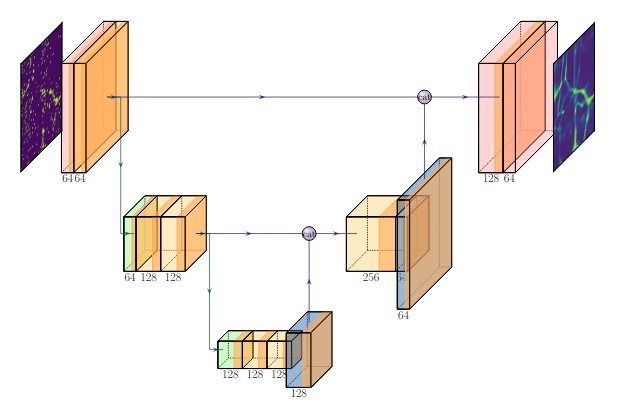
\includegraphics[width=\textwidth]{unet.png}
  \caption{U-net architecture used for the generator in \cite{superresolving-halos}. Note the three levels of hierarchy in generation.}
  \label{unet}
\end{figure}

Another hyperparameter in Schaurecker et al. is the objective function. Schaurecker et al. uses a regularization term suggested by \cite{GAN-regularization}
\[L(G, D) = \mathbb E [\log D(a, b) | (a, b) \in R] + \mathbb E [\log(1 - D(G(a))) | a \in A] + \gamma \mathbb E [\nabla D(a, b) | (a, b) \in R]\]
with \(\gamma = 5\). It is unclear if this hyperparameter will transfer to a different space.
